\documentclass[12pt]{article}

\pagestyle{empty}
\setcounter{secnumdepth}{2}

\topmargin=0cm
\oddsidemargin=0cm
\textheight=22.0cm
\textwidth=16cm
\parindent=0cm
\parskip=0.15cm
\topskip=0truecm
\raggedbottom
\abovedisplayskip=3mm
\belowdisplayskip=3mm
\abovedisplayshortskip=0mm
\belowdisplayshortskip=2mm
\normalbaselineskip=12pt
\normalbaselines

\usepackage{graphicx}
\usepackage{float}

\begin{document}

\vspace*{0.5in}
\centerline{\bf\Large Requirements Document}

\vspace*{0.5in}
\centerline{\bf\Large Team PB-PI}

\vspace*{0.5in}
\centerline{\bf\Large February 11, 2018}

\vspace*{1.5in}
\begin{table}[htbp]
\caption{Team}
\begin{center}
\begin{tabular}{|r | c|}
\hline
Name & ID Number \\
\hline\hline
Alissa Bellerose & 27377320 \\
Sabrina D'Mello & 27739486 \\
Melanie Damilig & 40032420 \\
Tobi Decary-Larocque & 27407645 \\
Zain Farookhi & 26390684 \\
Giulia Gaudio & 27191766 \\
Jason Kalec & 40009464 \\
Damian Kazior & 40016168 \\
Johnny Mak & 40002140 \\
Philip Michael & 40004861 \\
Ramez Nicolas Nahas & 26718108 \\
Steven Tucci & 40006014 \\
Shunyu Wang & 40043915 \\
\hline
\end{tabular}
\end{center}
\end{table}

\clearpage

\section{System}

\subsection{Purpose}
The purpose of this document is to outline the requirements for the myMoney application. It provides direction and background to anyone involved in developing, testing and maintaining the system.

The intended audience of this document is described in table~\ref{tab:intended_audience}.

\begin{table}[htbp]
\caption{Intended audience}
\label{tab:intended_audience}
\begin{center}
  \begin{tabular}{|l|p{10cm}|}
      \hline
      Reader & Reason\\
      \hline\hline
      Users/Customers & Give feedback\\
      \hline
      System Developers & Understand the functionality and properties the application contains\\
      \hline
      Testers & Test the system\\
      \hline
      User Manual Writers & Source material for manuals\\
      \hline
      Project Team & Keep track of status of project\\
      \hline
  \end{tabular}
\end{center}
\end{table}

\subsection{Business Goals}
Our customers are money-conscious people who would benefit from a system that makes it easier to track how their money moves.

There currently is no efficient way for people to stay on top of their finances. To do it, they must rely on bank statements and receipts, and must learn to navigate through a variety of interfaces to keep track of different accounts. 

Our system makes it easier for people to control their finances, by allowing them for example to record cash deposits/withdrawals and track income/expenses across various accounts, all in one place.

\section{Domain Concepts}

\begin{figure}[h]
  \centering
  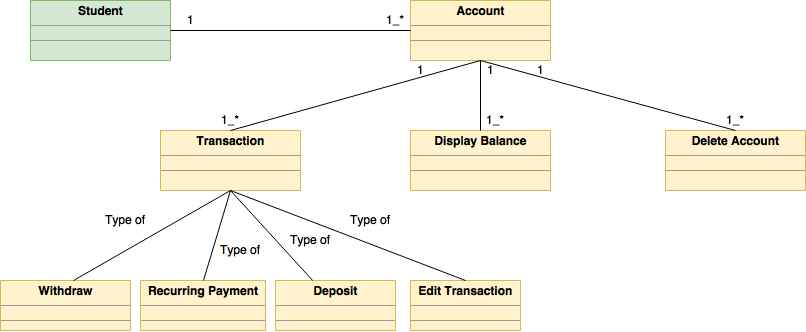
\includegraphics[width=130mm,natwidth=806,natheight=332]{Domain_model.png}
  \caption{Domain model}
  \label{fig:model}
\end{figure}
 
 
 
\begin{table}[H]
\caption{Main domain concepts}
\begin{center}
\begin{tabular}{|p{3cm}|p{12cm}|}
\hline
Concept & Description \\
\hline\hline
Student & Main user of the system. Student manually keeps the system up to date by entering every transaction performed during his day to day activities.  \\
\hline
Deposit & An action performed by the student. Whenever they receive money, student indicates that amount in myMoney app as a deposit. \\
\hline
Withdrawal & Every time student spends money, withdrawal object is created. It can be a type of credit card purchase or paying a bill. \\
\hline
Bill & Cash payment that student performs. Amount of bill paid in cash must be entered manually. \\
\hline
Credit card & Indicate credit card purchase. Every credit card payment is manually entered into myMoney app. \\
\hline
\end{tabular}
\end{center}
\end{table}

\section{System overview}


The myMoney application is a simple personal funds management system. It tracks a user's deposits and expenses across different banks and accounts within these banks. System is maintained by the user and is not connected to any bank account.

\section{Actors}

\begin{table}[H]
  \caption{User groups}
  \begin{center}
    \begin{tabular}{|l|p{8cm}|c|}
      \hline
      User Group & Description & Number of Users\\
      \hline\hline
      Young adults & Student or adult at an early stage of their career & 1\\
      \hline
    \end{tabular}
  \end{center}
\end{table}

\section{Functional Requirements}
\begin{table}[H]
\caption{Functionalities}
  \begin{center}
    \begin{tabular}{|l|p{10cm}|}
      \hline
      Field & Description\\
      \hline\hline
      \bf ID & \bf {F1}\\
      \hline
      Version & 1\\
      \hline
      Feature & Transaction\\
      \hline
      Requirement & The system must be able to make a transaction from an account\\
      \hline
      Source & Team Brainstorm\\
      \hline
      Rationale & For a user to keep track of their budget, they must be able to record changes made within an account by adding transactions to said account\\
      \hline
      Priority & Must\\
      \hline
      Status & Implemented\\
      \hline
      Traces to use cases & Withdrawal \& Deposit Amount\\
      \hline
    \end{tabular}
  \end{center}
\end{table}
\begin{table}
  \begin{center}
    \begin{tabular}{|l|p{10cm}|}
      \hline
      \bf ID & \bf {F2}\\
      \hline
      Version & 1\\
      \hline
      Feature & Transaction\\
      \hline
      Requirement & The user may only enter a numeric entry as input for the amount to deposit or withdraw\\
      \hline
      Source & User\\
      \hline
      Rationale & Monetary value is numerical, therefore we must ensure that input is valid, for system to accept the input\\
      \hline
      Priority & Must\\
      \hline
      Status & Proposed\\
      \hline
      Traces to use cases & Withdrawal,  Deposit Amount \& Edit Transaction\\
      \hline
    \end{tabular}
  \end{center}
\end{table}
\begin{table}
  \begin{center}
    \begin{tabular}{|l|p{10cm}|}
      \hline
      \bf ID & \bf {F3}\\
      \hline
      Version & 1\\
      \hline
      Feature & Transaction\\
      \hline
      Requirement & Transaction should require confirmation before being processed\\
      \hline
      Source & Team Brainstorm\\
      \hline
      Rationale & To ensure transaction is properly entered, system will prompt the user to confirm the transaction after inputting an amount\\
      \hline
      Priority & Must\\
      \hline
      Status & Proposed\\
      \hline
      Traces to use cases & Withdrawal \& Deposit Amount\\
      \hline
    \end{tabular}
  \end{center}
\end{table}

\section{Non-functional Requirements}

\begin{table}[H]
  \caption{Non-functional requirements}
  \begin{center}
    \begin{tabular}{|l|p{10cm}|}
      \hline
      Field & Description\\
      \hline\hline
      \bf ID & \bf {D1}\\
      \hline
      Ver & 1\\
      \hline
      Requirement & All documentation will be found within the source code in the repository\\
      \hline
      Source & Team Brainstorm\\
      \hline
      Rationale & All documents should be centrally located and accessible by all team members\\
      \hline
      Priority & Want\\
      \hline
      Status & Implemented\\
      \hline
      Traces to use cases & -\\
      \hline\hline
      \bf ID & \bf {S1}\\
      \hline
      Ver & 1\\
      \hline
      Requirement & User's financial information needs to be encrypted in database\\
      \hline
      Source & Organizer\\
      \hline
      Rationale & System will be handling sensitive information about the user's finances. Data such as account numbers will need to be encrypted for protection\\
      \hline
      Priority & Must\\
      \hline
      Status & Proposed\\
      \hline
      Traces to use cases & -\\
      \hline
    \end{tabular}
  \end{center}
\end{table}

\break
\section{Use Cases}

\subsection{Overview}

\begin{figure}[h!]
  \centering
  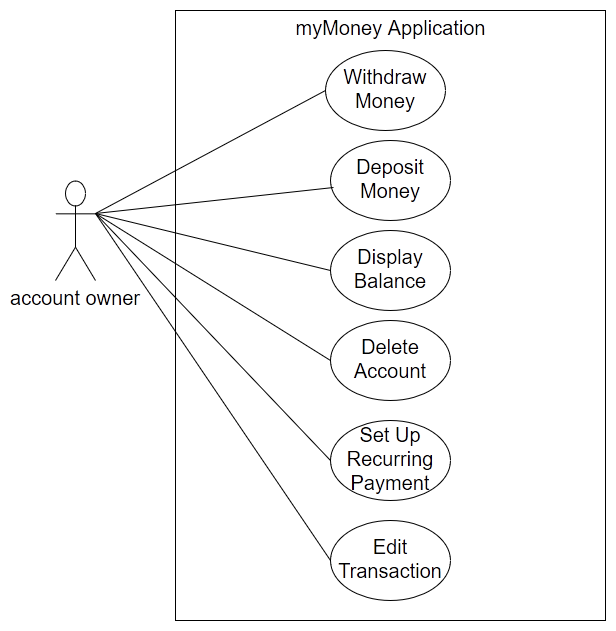
\includegraphics[width=110mm,natwidth=616,natheight=631]{Use_Case_Diagram.png}
  \caption{Use Case Diagram}
  \label{fig:use_case_diagram}
\end{figure}

\subsubsection{Use Case 1} \label{uc:1}

\noindent
{\bf ID}\\
UC-MWA-001\\
    
\noindent
{\bf Name}\\
Withdraw money.\\

\noindent
{\bf Goal}\\
The user withdraws an amount of money from the selected account.

\noindent
{\bf Actors}\\
Primary Actor - owner of the account.

\noindent
{\bf Precondition}\\
User is the owner of the account.

\noindent
{\bf Main Scenario}\\
\vspace*{-0.2in}
\begin{enumerate}
  \item Primary actor indicates to withdraw an amount from a selected account.
  \item System verifies the account exists.
  \item System prompts primary actor for the amount to withdraw.
  \item User enters amount to withdraw.
  \item System verifies that the account contains sufficient funds.
  \item System prompts user for confirmation.
  \item User confirms.
  \item System subtracts amount of money requested from selected account, confirms withdrawal.
  \item Use case ends succesfully.
\end{enumerate}

\noindent
    {\bf Exceptions}\\
    \vspace*{-0.2in}
\begin{itemize}
    \item[2a)] Account does not exist.
    \item[5a)] Account has an empty or negative balance.
    \item[5b)] Account contains insufficient funds.
\end{itemize}
    

\noindent
{\bf Postcondition}\\
The amount is subtracted from the selected account.

\noindent
{\bf Priority}\\
Critical.   

%\noindent
%{\bf Traces to Test Cases}\\
%Add when test cases done.

\subsubsection{Use Case 2} \label{uc:2}

\noindent
{\bf ID}\\
UC - MDA - 002

\noindent
{\bf Name}\\
Deposit Money.

\noindent
{\bf Goal}\\
User succesfully deposits an amount of money to the selected account.

\noindent
{\bf Actors}\\
Primary Actor - owner of the account.

\noindent
{\bf Precondition}\\
User is owner of the account.

\noindent
{\bf Main Scenario}\\
\vspace*{-0.2in}
\begin{enumerate}
  \item Primary actor indicates to deposit an amount to a selected account.
  \item System verifies that the account exists.
  \item System prompts user to enter amount to deposit.
  \item System verifies amount is valid.
  \item System adds amount of money deposited to selected account and confirms.
  \item Use case ends succesfully.
\end{enumerate}

\noindent
    {\bf Exceptions}\\
    \vspace{-0.2in}
    \begin{itemize}
    \item[2a)] Account does not exist.
    \item[4a)] Amount is zero or negative.
    \end{itemize}

\noindent
{\bf Postcondition}\\
The amount is added to the selected account.

\noindent
{\bf Priority}\\
Critical.

%\noindent
%{\bf Traces to Test Cases}\\
%Add when test cases done.

\subsubsection{Use Case 3} \label{uc:3}

\noindent
{\bf ID}\\
UC - DBA - 003    

\noindent
{\bf Name}\\
Display Balance.

\noindent
{\bf Goal}\\
Display balance of chosen account to user.

\noindent
{\bf Actors}\\
Primary Actor - Owner of the account

\noindent
{\bf Precondition}\\
Account exists.

\noindent
{\bf Main Scenario}\\
\vspace*{-0.2in}
\begin{enumerate}
\item Primary Actor selects account to be displayed.
  \item System retrieves account information from database.
\item System displays balance.
\end{enumerate}

\noindent
{\bf Exceptions}\\
\vspace*{-0.2in}
\begin{itemize}
\item[1a)] Account does not exist.
\item[2a)] System cannot retrieve data for chosen account.
\end{itemize}

\noindent
{\bf Postcondition}\\
Account balance is displayed for user.

\noindent
{\bf Priority}\\
Critical.

\subsubsection{Use Case 4} \label{uc:4}

\noindent
{\bf ID}\\
UC - DA - 004

\noindent
{\bf Name}\\
Delete Account.

\noindent
{\bf Goal}\\
User deletes selected account.

\noindent
{\bf Actors}\\
Primary Actor - owner of the account.

\noindent
{\bf Precondition}\\
User is owner of the account.
At least one account exists.

\noindent
{\bf Main Scenario}\\
\vspace*{-0.2in}
\begin{enumerate}
\item User indicates to delete the selected account.
\item System verifies that the selected account exists
\item System prompts the user for confirmation.
\item User confirms.
\item System deletes selected account.
  \item Use case ends successfully.
\end{enumerate}

\noindent
    {\bf Exceptions}\\
    \vspace{-0.2in}
    \begin{itemize}
    \item[1a)] There is no account.
    \end{itemize}

\noindent
{\bf Postcondition}\\
Selected account is deleted.

\noindent
{\bf Priority}\\
Critical.

\subsubsection{Use Case 5} \label{uc:5}

\noindent
{\bf ID}\\
UC - SRA - 002

\noindent
{\bf Name}\\
Set Up Recurring Payment.

\noindent
{\bf Goal}\\
User can set up recurring payments.

\noindent
{\bf Actors}\\
Primary Actor - owner of the account.

\noindent
{\bf Precondition}\\
User is owner of the account.
At least one account exists.

\noindent
{\bf Main Scenario}\\
\vspace*{-0.2in}
\begin{enumerate}
  \item User indicates to set up a recurring payment.
  \item User chooses the appropriate account.
  \item System prompts user to enter the amount of payment.
  \item User enters amount of payment.
  \item System verifies amount is valid.
  \item User selects start date.
  \item User selects payment frequency.
  \item System prompts user for confirmation.
  \item User confirms.
  \item Use case ends succesfully.
\end{enumerate}

\noindent
    {\bf Exceptions}\\
    \vspace{-0.2in}
    \begin{itemize}
    \item[1a)] There is no account.
    \item[5a)] Amount is zero or negative.
    \item[9a)] User cancels or does not confirm.
    \end{itemize}

\noindent
{\bf Postcondition}\\
System records recurring payment information and initiates \underline{Money Withdrawal} accordingly.

\noindent
{\bf Priority}\\
Critical.

\subsubsection{Use Case 6} \label{uc:6}

\noindent
{\bf ID}\\
UC - ETR - 006

\noindent
{\bf Name}\\
Edit transaction.

\noindent
{\bf Goal}\\
User can modify an existing transaction.

\noindent
{\bf Actors}\\
Primary Actor - owner of the account.

\noindent
{\bf Precondition}\\
User is owner of the account.
At least one account exists.
At least one transaction has been saved.

\noindent
{\bf Main Scenario}\\
\vspace*{-0.2in}
\begin{enumerate}
  \item User indicates to modify a transaction.
  \item User chooses the appropriate account.
  \item User selects transaction to modify.
  \item System prompts user for confirmation.
  \item User confirms.
  \item User enters new amount and confirms.
  \item System prompts user for confirmation with details.
  \item User confirms.
  \item Use case ends succesfully.
\end{enumerate}

\noindent
    {\bf Exceptions}\\
    \vspace{-0.2in}
    \begin{itemize}
    \item[2a)] There is no account.
    \item[3a)] There are no transactions for selected account.
    \item[6a)] Amount is not valid.
    \end{itemize}

\noindent
    {\bf Postcondition}\\
    Transaction has been altered to reflect changes.

\noindent
{\bf Priority}\\
Critical.

%\noindent
%{\bf Traces to Test Cases}\\
%Add when test cases done.

\section{Constraints}
\begin{table}[H]
\caption{System Constraints}
  \begin{center}
    \begin{tabular}{|l|p{10cm}|}
      \hline
      Field & Description\\
      \hline\hline
      ID & C1\\
      \hline
      Ver & 1\\
      \hline
      Constraint & The application must run on any well-known desktop operating system including Apple \& Windows OSs\\
      \hline
      Source & Team Brainstorm\\
      \hline
      Rationale & Serve all users across different operating systems\\
      \hline
      Priority & Must\\
      \hline
      Status & Proposed\\
      \hline
      Traces to use cases & All use cases with a desktop interface\\
      \hline
    \end{tabular}
  \end{center}
\end{table}

\section{Solution ideas}
\begin{table}[H]
\caption{Solution Idea I}
  \begin{center}
    \begin{tabular}{|l|p{10cm}|}
      \hline
      Field & Description\\
      \hline\hline
      ID & SI1\\
      \hline
      Ver & 1\\
      \hline
      Solution idea & Total amount of withdrawals \& deposits could be displayed using charts\\
      \hline
      Source & Team Brainstorm\\
      \hline
      Rationale & When evaluating interesting budgeting applications, use of charts offers quick and clear overview of the user's financial situation\\
      \hline
      Traces to use cases & Display balance\\
      \hline
    \end{tabular}
  \end{center}
\end{table}

\section{Acronyms and Abbreviations}
\begin{table}[H]
  \begin{tabular}{l l}
    \bf{C} x & Constraint x\\
    \bf{ChAc} & Chequing Account\\
    \bf{D} x & Documentation x\\
    \bf{DBA} & Display Balance\\
    \bf{F} x & Functionality x\\
    \bf{MDA} & Money Deposit\\
    \bf{MWA} & Money Withdrawal\\
    \bf{SavAc} & Savings Account\\
    \bf{S} x & Security x\\
    \bf{SI} x & Solution Idea x\\
  \end{tabular}
\end{table}

\section{References}
We obtained an example \textit{User Requirements Document} from the website http://www.soberit.hut.fi/T-76.115/05-06/ohjeet/template/requirements.html.

\appendix

%\section{Description of File Format: Tasks}

%Describe input file format.

%\section{Description of File Format: Persons}

%Describe output file format.

\end{document}
